% Chapter Template

% Main chapter title
%\chapter[toc version]{doc version}
\chapter{Chapter Title Here}

% Short version of the title for the header
%\chaptermark{version for header}

% Chapter Label
% For referencing this chapter elsewhere, use \ref{ChapterTemplate}
\label{ChapterTemplate}

% Write text in here
% Use \subsection and \subsubsection to organize text

Welcome to the tutorial on how to use this thesis model. This is not to teach
you how to use \LaTeX. For that read a tutorial. But this aims to teach you how
to do the basic stuff you will need in order to produce a decent document.
We can start with a section and a section epigraph:

\section{Citations}
\epigraph{Python is a truly wonderful language. When somebody comes up with a good idea it takes about 1 minute and five lines to program something that almost does what you want. Then it takes only an hour to extend the script to 300 lines, after which it still does almost what you want.}{Dr. Jack Jansen,  maintainer of MacPython}

You can add extra info to you references, like~\cite[section 3]{Fienup1982}. You
can also call them by author, like saying~\citet{Fienup1982}\unsure{You can make
personal notes like this}.

Also a random displayquote thing:

\begin{displayquote}
    How can we image an object that's behind or enclosed on a medium where light does not propagate trivially? How can we manipulate light propagating in these media?
\end{displayquote}

\section{Figures}

Let us start with a figure with two subfigures like in~\ref{fig:FCUPfatCat}.
\begin{figure}
	\centering
	\begin{subfigure}{.49\textwidth}
  		\centering
          
\includegraphics[width=.95\linewidth]
            {ChapterTemplate/20160517_123603.jpg}
  		\caption{FCUP's fat cat doing what cats do.}
	\end{subfigure}%
	\hfill
	\begin{subfigure}{.49\textwidth}
  		\centering
          
\includegraphics[width=.95\linewidth]
            {ChapterTemplate/20160517_123609.jpg}
 		 \caption{FCUP's fat cat resting.}
	\end{subfigure}
	\caption{\label{fig:FCUPfatCat}FCUP's fat cat.}
\end{figure}


Or two figures side by side like~\ref{fig:FCUPfatcatSide1}
and~\ref{fig:FCUPfatcatSide2}.

\begin{figure}
\centering
\begin{minipage}{.49\textwidth}
  \centering
  
\includegraphics[width=.95\linewidth]{ChapterTemplate/20160517_123603.jpg}
  \captionof{figure}{\label{fig:FCUPfatcatSide1}FCUP's fat cat doing what cats do.}
\end{minipage}%
\hfill
\begin{minipage}{.49\textwidth}
  \centering
  
\includegraphics[width=.95\linewidth]{ChapterTemplate/20160517_123609.jpg}
  \captionof{figure}{\label{fig:FCUPfatcatSide2}FCUP's fat cat.}
\end{minipage}
\end{figure}


Or a figure with some text on the side, like~\ref{fig:FCUPfatcatSide3}, or even
a figure wrapped around in text, as seen on Figure~\ref{fig:FCUPfatcatSide4}.

\begin{figure}
\centering
\begin{minipage}{.49\textwidth}
  And here we have some text related to this image. The text can occupy the same space as the image would normally do.
\end{minipage}%
\hfill
\begin{minipage}{.49\textwidth}
  \centering
  
\includegraphics[width=.95\linewidth]{ChapterTemplate/20160517_123609.jpg}
  \captionof{figure}{\label{fig:FCUPfatcatSide3}FCUP's fat cat.}
\end{minipage}
\end{figure}

\textcolor{red}{This is where the float goes with text wrapping around it. You
may embed tabular environment inside wraptable environment and customize as you
like:} Ultrices dui sapien eget mi proin sed libero. Ornare lectus sit amet est
placerat in egestas erat imperdiet. Tortor dignissim convallis aenean et. Quam
adipiscing vitae proin sagittis nisl rhoncus mattis. Vivamus at augue eget arcu
dictum varius duis. Cursus turpis massa tincidunt dui.
\begin{wrapfigure}{r}{8cm}
    % If you find figures split between two pages, use the uppercase L or R, to
    % let the wrapped figure be a float object that can move through the page.
    \centering
    
\includegraphics[width=7cm]{ChapterTemplate/20160517_123609.jpg}
    \captionof{figure}{\label{fig:FCUPfatcatSide4}FCUP's fat cat.}
  \end{wrapfigure}
Leo in vitae turpis massa sed. Tempor orci eu lobortis elementum. Turpis egestas
integer eget aliquet nibh praesent tristique magna. Sed blandit libero volutpat
sed cras ornare arcu dui. Feugiat sed lectus vestibulum mattis ullamcorper velit
sed ullamcorper. Interdum velit euismod in pellentesque massa placerat duis
ultricies lacus. Ac ut consequat semper viverra nam. Dis parturient montes
nascetur ridiculus mus. Mattis pellentesque id nibh tortor.

\subsection{SVGs}
How to make a \LaTeX\ document with vector images, where the text in the images
has exactly the same font and size as in normal text? This article describes how
this is done using the `PDF/EPS/PS + LaTeX' output feature of Inkscape 0.48.
Inkscape can export the graphics to PDF/EPS/PS, and the text to a \LaTeX\ file.
When the \LaTeX\ file is input in the \LaTeX\ document, the PDF/EPS/PS image is
included with overlaid text. Because typesetting of the text is done by \LaTeX,
\LaTeX\ commands can be used in images, such as writing equations, references
and shorthand macros.

\emph{(requires Inkscape version 0.48 or higher; this document discusses features up to Inkscape 0.49)}

\begin{figure}
    \centering
      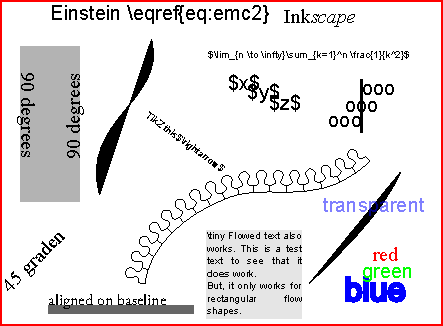
\includegraphics[width=0.5\columnwidth]{ChapterTemplate/image-normal.pdf}
      \caption[The test SVG image, as it is seen in Inkscape]
      {The test SVG image, as it is seen in Inkscape (exported to PDF
      \emph{without} \LaTeX\ option).}
      \label{fig:normal}
\end{figure}

\begin{figure}
\centering
    \includesvg[width=0.8\columnwidth]{image}
    \caption{The test image, exported to PDF \emph{with} \LaTeX\ option.}
    \label{fig:pdflatex}
\end{figure}

\begin{equation}
    \label{eq:emc2}
    E = mc^{2}
\end{equation}

\subsubsection{Automatic export}

(`write18' must be enabled, see the {\small\verb|epstopdf|} package
documentation. Add {\small\verb|-shell-escape|} to the command line when calling
{\small\verb|pdflatex|}. \textcolor{red}{And inkscape must be discoverable by the
OS}),

Whenever the SVG file is updated, it is possible to have \LaTeX\ automatically call Inkscape to export the image to PDF and \LaTeX\ again. This simplifies the workflow to
\begin{itemize}
	\item Modify the SVG image in Inkscape;
	\item Save the SVG (Ctrl+S, no need to export to PDF);
	\item Recompile \LaTeX\ document. pdf\LaTeX\ will notice the SVG file has changed, and will automatically do the export for you.
\end{itemize}

\section{Math}

The following equation uses a custom mathematical operator defined in line 88
of preamble.tex:
\begin{equation}
\begin{aligned}
            \meshgrid_{\mathbf{x}_{1},\mathbf{x}_{2}}\mathbf{x}_{1}&=
            \begin{bmatrix}a_{1} & b_{1} & c_{1}\\
            a_{1} & b_{1} & c_{1}
\end{bmatrix}\\
            \meshgrid_{\mathbf{x}_{1},\mathbf{x}_{2}}\mathbf{x}_{2}&=
            \begin{bmatrix}a_{2} & a_{2} & a_{2}\\
            b_{2} & b_{2} & b_{2}
\end{bmatrix}
\end{aligned}
\end{equation}

The following equation uses the custom ceil and floor operator defined in line 86 of the stock preamble.tex:

\begin{equation}
x = \floor*{\frac{y}{2}} + \ceil*{\frac{w}{2}}
\end{equation}


And this is an equation with multiple lines:
\begin{equation}
\begin{aligned}
&I_{0}=I^{\prime}+I^{\prime\prime}\cos(\varPsi)   \\
&I_{\pi/2}=-I^{\prime\prime}\sin(\varPsi)                \\
&I_{\pi}=I^{\prime}-I^{\prime\prime}\cos(\varPsi)   \\
&I_{3\pi/2}=I^{\prime\prime}\sin(\varPsi)
\end{aligned}
\end{equation}

And this is some random Python code:

\begin{lstlisting}[style = Python]
def Hello():
    """
      Meaningful docstring with in-depth explanation of this function
    """
    print(``Hello World !!'')

if __name__ == '__main__':
    Hello()
\end{lstlisting}
\section{Abreviations}

Use acronyms like this: \ac{ann}